%%
% This is an Overleaf template for presentations
% using the TUM Corporate Desing https://www.tum.de/cd
%
% For further details on how to use the template, take a look at our
% GitLab repository and browse through our test documents
% https://gitlab.lrz.de/latex4ei/tum-templates.
%
% The tumbeamer class is based on the beamer class.
% If you need further customization please consult the beamer class guide
% https://ctan.org/pkg/beamer.
% Additional class options are passed down to the base class.
%
% If you encounter any bugs or undesired behaviour, please raise an issue
% in our GitLab repository
% https://gitlab.lrz.de/latex4ei/tum-templates/issues
% and provide a description and minimal working example of your problem.
%%

%\PassOptionsToClass{onlytextwidth}{beamer}

\documentclass[
  german,            % define the document language (english, german)
  aspectratio=169,    % define the aspect ratio (169, 43)
  % handout=2on1,       % create handout with multiple slides (2on1, 4on1)
  % partpage=false,     % insert page at beginning of parts (true, false)
  % sectionpage=true,   % insert page at beginning of sections (true, false)
]{tumbeamer}


% load additional packages
\usepackage{booktabs}
\usepackage{graphicx}
\usepackage{tikz}
\usepackage{url}
\usepackage{pgf}
\usepackage{pgfplots}
\usepackage{hyperref}
\usepackage{pmboxdraw}
\usepackage{float}
\usepackage{babel}[ngerman]
\usepackage{csquotes}[autostyle]
\usepackage[useregional]{datetime2}
\usepackage[cache=true]{minted}
\usemintedstyle{borland}
\usepackage{listings}
\usepackage{siunitx}


% tikz  
\usetikzlibrary{fit, matrix, calc, arrows, arrows.meta, positioning, patterns, bending, overlay-beamer-styles}

% minted
\setminted{
	fontsize=\small, 
	frame=none,
	breaklines=true,
	style=pastie,
	tabsize=4, 
	autogobble,
}

% listings
\lstset{        basicstyle=\ttfamily,
	numbers=left,
	stepnumber=1,
	showstringspaces=false,
	tabsize=4,
	breaklines=true,
	breakatwhitespace=false,
	frame=single}

% xcolor
\definecolor{altblue}{HTML}{44C8F5}
\definecolor{altyellow}{HTML}{FFE600}
\definecolor{altgreen}{HTML}{26E600}
\definecolor{altmagenta}{HTML}{EC008C}

\captionsetup{labelformat=empty}

% image path
\graphicspath{ {./resources/} }

% beamer
\setbeamercolor{footnote}{fg=black}
\setbeamercolor{footnote mark}{fg=black}
\renewcommand{\thempfootnote}{\arabic{mpfootnote}}

% presentation metadata
\title{Übung 04: Rekursion und \\Calling Convention}
\subtitle{Einführung in die Rechnerarchitektur}
\author{Niklas Ladurner}

\institute{\theChairName\\\theDepartmentName\\\theUniversityName}
\date{\DTMdisplaydate{2025}{11}{7}{-1}}

\footline{\insertauthor~|~\insertshorttitle~|~\insertshortdate}


% macro to configure the style of the presentation
\TUMbeamersetup{
  title page = TUM tower,         % style of the title page
  part page = TUM toc,            % style of part pages
  section page = TUM toc,         % style of section pages
  content page = TUM more space,  % style of normal content pages
  tower scale = 1.0,              % scaling factor of TUM tower (if used)
  headline = TUM threeliner,      % which variation of headline to use
  footline = TUM default,         % which variation of footline to use
  % configure on which pages headlines and footlines should be printed
  headline on = {title page},
  footline on = {every page, title page=false},
}

% available frame styles for title page, part page, and section page:
% TUM default, TUM tower, TUM centered,
% TUM blue default, TUM blue tower, TUM blue centered,
% TUM shaded default, TUM shaded tower, TUM shaded centered,
% TUM flags
%
% additional frame styles for part page and section page:
% TUM toc
%
% available frame styles for content pages:
% TUM default, TUM more space
%
% available headline options:
% TUM empty, TUM oneliner, TUM twoliner, TUM threeliner, TUM logothreeliner
%
% available footline options:
% TUM empty, TUM default, TUM infoline


\begin{document}

\maketitle

\begin{frame}[c, fragile]{}{}
	\begin{center}
		\LARGE  Keine Garantie für die Richtigkeit der Tutorfolien.

		\Large Bei Unklarheiten/Unstimmigkeiten haben VL/ZÜ-Folien recht!
	\end{center}
\end{frame}

\begin{frame}[c]{Stack}{}
	\vspace*{-1cm}
	\begin{columns}[c]
		\begin{column}{0.5\textwidth}
			\begin{itemize}
				\item Speicherbereich für lokale Variablen
				\item wächst von hohen Adressen zu niedrigen Adressen
				\item Anpassen des Stackpointers durch Beschreiben des \texttt{sp}-Registers
				\item alles an Adressen \textless{} \texttt{sp} ungeschützt
				\item besonders wichtig für Rekursion (Stackframes)
			\end{itemize}
		\end{column}%
		\begin{column}{0.4\textwidth}
			\begin{center}
				\resizebox{\textwidth}{!}{
					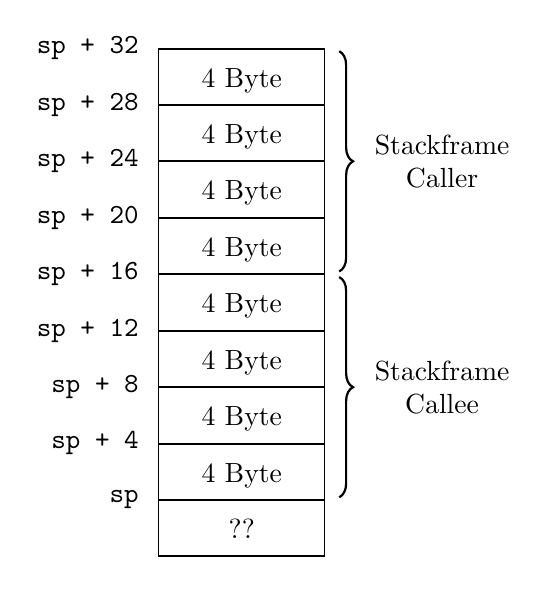
\begin{tikzpicture}
						\tikzset{
							label/.style = {font={\ttfamily}, anchor=west},
							biglabel/.style = {text width=2cm, align=center, anchor=west},
							arrow/.style={Latex-, thick},
							matstyle/.style={ matrix of nodes, ampersand replacement=\&, nodes={draw, minimum width=6em, minimum height=2em, text height=1em, text depth=0.25em, align=center, anchor=south}, column sep=-\pgflinewidth},
							bbrace/.style={decorate,decoration={brace,amplitude=5pt,raise=0.5em}, rotate=90, thick},
						}

						\matrix[matstyle] (mat) {
							4 Byte%
							\\4 Byte%
							\\4 Byte%
							\\4 Byte%
							\\4 Byte%
							\\4 Byte%
							\\4 Byte%
							\\4 Byte%
							\\??%
							\\
						};

						\foreach \x/\l in {1/sp + 32, 2/sp + 28, 3/sp + 24, 4/sp + 20, 5/sp + 16, 6/sp + 12, 7/sp + 8, 8/sp + 4, 9/sp}
							{
								\node[label, left=0.125cm of mat-\x-1.north west, anchor=east] (addr) {\l};
							}


						\draw [bbrace] ($(mat-1-1.north east) + (-1pt, 0)$) -- ($(mat-4-1.south east) + (1pt, 0)$) node[midway,xshift=1em,biglabel]{Stackframe\\Caller};

						\draw [bbrace] ($(mat-5-1.north east) + (-1pt, 0)$) -- ($(mat-8-1.south east) + (1pt, 0)$) node[midway,xshift=1em,biglabel]{Stackframe\\Callee};

					\end{tikzpicture}
				}
			\end{center}
		\end{column}
	\end{columns}
\end{frame}

\begin{frame}[c, fragile]{Caller und Callee (1)}{}
	\begin{center}
		\begin{tikzpicture}
			\def\arc{0.9cm}
			\def\spc{3.75*\arc}
			\def\lblspc{3cm}

			\tikzset{
				codebox/.style = {draw=none, inner sep=0pt},
				label/.style = {text width=4cm, align=center},
				arrow/.style={-Latex, thick},
			}

			\node[codebox, anchor=north, visible on=<1->] (caller) {\begin{minipage}{0.25\textwidth}
					\begin{minted}{gas}
					main:
						li a0, 3
						li a1, 5
						jal multiply
						addi a0, a0, 1 
						ret
				\end{minted}
				\end{minipage}};

			\node[codebox, right=\spc of caller.north east, anchor=north, visible on=<1->] (callee) {\begin{minipage}{0.3\textwidth}
					\begin{minted}{gas}
					multiply:
						mul a0, a0, a1
						ret
				\end{minted}
				\end{minipage}};

			\node[label, below=of caller, visible on=<1->] (lbl1) {\textbf{Caller}\\(aufrufende Funktion)};
			\node[label, right=\spc of lbl1.north east, anchor=north, visible on=<1->] {\textbf{Callee}\\(aufgerufene Funktion)};


			\coordinate (jexit) at ($(caller.north east) +(-0.8cm, -1.1cm)$) {};
			\coordinate (jentry) at ($(jexit) +(2*\arc, \arc)$) {};
			\draw[arrow, visible on=<2->] (jexit) to[bend left] (jentry);

			\node[draw=none, visible on=<2->] (ra)  at ($(caller.north west) +(-0.3cm, -1.89cm)$) {\texttt{ra}};
			\draw[arrow, visible on=<2->](ra) -- ++ (1cm, 0);

			\coordinate (rexit) at ($(callee.north west) +(0.75cm, -1.05cm)$) {};
			\coordinate (rentry) at ($(rexit) +(-2*\arc, -\arc)$) {};
			\draw[arrow, visible on=<3->] (rexit) to[bend left] (rentry);
		\end{tikzpicture}
	\end{center}
\end{frame}

\begin{frame}[c, fragile]{Caller und Callee (2)}{}
	\begin{columns}[c]
		\hspace*{0.25cm}
		\begin{column}{0.5\textwidth}
			\begin{minted}[fontsize=\scriptsize]{gas}
caller:
# aufrufende Funktion (Caller)

# wir speichern die Rücksprungadresse auf 
# den Stack -> ra ist Caller-saved!
addi sp, sp, -16
sw ra, 0(sp)

# ... irgendwas, was t0 verwendet

# da t0 caller-saved ist, müssen wir uns
# t0 absichern, falls wir den Inhalt später
# noch brauchen
sw t0, 4(sp)
# ...
jal ra, callee  # Sprung zur Unterfunktion
# ...
lw t0, 4(sp)
# ... wieder irgendwas mit t0
lw ra, 0(sp)
        \end{minted}
		\end{column}
		\begin{column}{0.5\textwidth}
			\begin{minted}[fontsize=\scriptsize]{gas}
addi sp, sp, 16
jalr zero, 0(ra)

callee:
# aufgerufene Funktion (Callee)

# hier dürfen wir t0-t6 bspw. verändern
# falls wir s0-s6 verändern wollen,
# müssen sie gesichert werden:
addi sp, sp, -16
sw s2, 0(sp)
sw s3, 4(sp)

# s2, s3 können jetzt verwendet werden!

lw s2, 0(sp)
lw s3, 4(sp)
addi sp, sp, 16
jalr zero, 0(ra)
      \end{minted}
		\end{column}
	\end{columns}
	\begin{center}
		\small{fürs Selbststudium :)}
	\end{center}
\end{frame}

\begin{frame}[c, fragile]{Calling Convention}{}
	\begin{itemize}
		\item \enquote{Aufrufkonvention} $\rightarrow$ lediglich eine Vereinbarung
		\item definiert Parameterübergabe, Rückgabe, Registersicherung, Stack etc.
		      \begin{enumerate}
			      \item Datentypen $\le$ 4 Byte in \texttt{a}-Register, sign-extension falls vorzeichenbehafteter Datentyp
			      \item Datentypen $=$ 8 Byte in zwei \texttt{a}-Registern, niedrigwertige Hälfte zuerst
			      \item Datentypen $>$ 8 Byte als Pointer auf Speicher (meist Caller-Stack)
			      \item Falls zu wenige Register: Übergabe über Stack
		      \end{enumerate}
		\item Stackpointer muss immer ein Vielfaches von 16 Byte sein!
	\end{itemize}
\end{frame}

\begin{frame}[c]{Register}{}
	\begin{center}
		{\rmfamily
			\begin{tabular}{|l|l|l|c|}
				\hline
				Register        & ABI Name       & Description                      & Saver  \\ \hline
				\texttt{x0}     & \texttt{zero}  & Hard-wired zero                  & ---    \\
				\rowcolor{altblue}
				\texttt{x1}     & \texttt{ra}    & Return address                   & Caller \\
				\texttt{x2}     & \texttt{sp}    & Stack pointer                    & Callee \\
				\texttt{x3}     & \texttt{gp}    & Global pointer                   & ---    \\
				\texttt{x4}     & \texttt{tp}    & Thread pointer                   & ---    \\
				\texttt{x5-x7}  & \texttt{t0-t2} & Temporaries                      & Caller \\
				\texttt{x8}     & \texttt{s0/fp} & Saved register/frame pointer     & Callee \\
				\texttt{x9}     & \texttt{s1}    & Saved register                   & Callee \\
				\rowcolor{altyellow}
				\texttt{x10-11} & \texttt{a0-1}  & Function arguments/return values & Caller \\
				\texttt{x12-17} & \texttt{a2-7}  & Function arguments               & Caller \\
				\rowcolor{altmagenta}
				\texttt{x18-27} & \texttt{s2-11} & Saved registers                  & Callee \\
				\rowcolor{altgreen}
				\texttt{x28-31} & \texttt{t3-6}  & Temporaries                      & Caller \\ \hline
			\end{tabular}
		}
	\end{center}
\end{frame}

\begin{frame}[c, fragile]{Rekursion (1)}{}
	\begin{columns}
		\begin{column}[c]{0.5\textwidth}
			\begin{itemize}
				\item Funktion die sich selbst aufruft
				\item Konzept: Berechnung aufteilen bis Basisfall erreicht
				\item jede rekursive Funktion kann auch iterativ implementiert werden ($\rightarrow$ Schleife)
				\item Beispiel Fibonacci-Folge: $f_n=f_{n-1}+f_{n-2}$,\\$f_1=1$, $f_0=0$

			\end{itemize}
		\end{column}%
		\begin{column}[c]{0.45\textwidth}
			\centering
			\resizebox{\textwidth}{!}{
			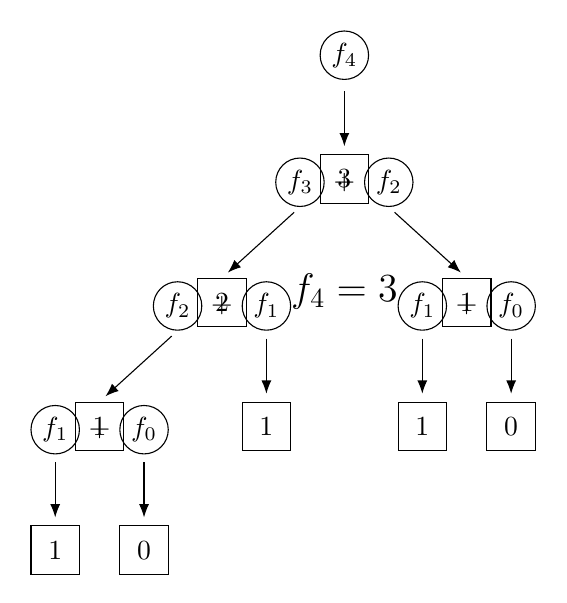
\begin{tikzpicture}
				\def\smallspace{0.9cm}
				\def\spread{1.1}


				\tikzset{
					arrow/.style={-Latex, shorten >=0.1cm, shorten <=0.1cm},
					matstyle/.style={matrix of nodes, inner sep=1pt, ampersand replacement=\&, nodes={draw=none, minimum width=1.5em, minimum height=1.5em}, column sep=-\pgflinewidth},
					c/.style = {circle,draw,solid,minimum width=1.75em,
							minimum height=1.75em},
					r/.style = {rectangle,draw,solid,minimum width=1.75em,
							minimum height=1.75em},
				}

				\matrix[matstyle, visible on=<2-13>] (top) {
				|[c]|$f_4$ \\
				};

				\matrix[matstyle, below=\smallspace of top, visible on=<3-12>] (f4) {
				|[c]|$f_3$\&$+$\&|[c]|$f_2$ \\
				};
				\draw[arrow, visible on=<3-13>](top.south) -- (f4.north);

				\matrix[matstyle, below=\smallspace of f4-1-1, xshift=-\spread*\smallspace, visible on=<4-8>] (f3) {
				|[c]|$f_2$\&$+$\&|[c]|$f_1$ \\
				};
				\draw[arrow, visible on=<4-12>](f4-1-1.south) -- (f3.north);

				\matrix[matstyle, below=\smallspace of f3-1-1, xshift=-\spread*\smallspace, visible on=<5-6>] (f22) {
				|[c]|$f_1$\&$+$\&|[c]|$f_0$ \\
				};
				\draw[arrow, visible on=<5-8>](f3-1-1.south) -- (f22.north);

				\visible<6>{
					\node[r, below=\smallspace of f22-1-1] (f221) {$1$};
					\node[r, below=\smallspace of f22-1-3] (f220) {$0$};
					\draw[arrow](f22-1-1.south) -- (f221.north);
					\draw[arrow](f22-1-3.south) -- (f220.north);
				}

				\node[r, below=\smallspace of f3-1-1, xshift=-\spread*\smallspace, visible on=<7-8>] (f22) {$1$};


				\node[r, below=\smallspace of f3-1-3, visible on=<8>] (f31) {$1$};
				\draw[arrow, visible on=<8>](f3-1-3.south) -- (f31.north);

				\node[r, below=\smallspace of f4-1-1, xshift=-\spread*\smallspace, visible on=<9-12>] (f22) {$2$};


				\matrix[matstyle, below=\smallspace of f4-1-3, xshift=\spread*\smallspace, visible on=<10-11>] (f2) {
				|[c]|$f_1$\&$+$\&|[c]|$f_0$ \\
				};
				\draw[arrow, visible on=<10-12>](f4-1-3.south) -- (f2.north);


				\node[r, below=\smallspace of f2-1-1, visible on=<11>] (f21) {$1$};
				\node[r, below=\smallspace of f2-1-3, visible on=<11>] (f20) {$0$};

				\draw[arrow, visible on=<11>](f2-1-1.south) -- (f21.north);
				\draw[arrow, visible on=<11>](f2-1-3.south) -- (f20.north);
				
				\node[r, below=\smallspace of f4-1-3, xshift=\spread*\smallspace, visible on=<12>] (f22) {$1$};
				
				\node[r, below=\smallspace of top, visible on=<13>] (f4) {$3$};
				
				
				\node[draw=none, visible on=<14>, font={\Large}] at (0,-3) {$f_4=3$};
			\end{tikzpicture}
		}
	\end{column}
	\end{columns}

\end{frame}

\begin{frame}[c, fragile]{Rekursion (2)}{}
	\begin{columns}[c]
		\begin{column}{0.4\linewidth}
			\begin{lstlisting}
fun:
  addi sp, sp, -8
  sw ra, 0(sp)
  sw a0, 4(sp)
  beq a0, zero, end
  addi a0, a0, -1
  jal fun
end:
  lw ra, 0(sp)
  addi sp, sp, 8
  jalr zero, 0(ra)
      \end{lstlisting}
			\small \textbf{Achtung}: 8 Byte nicht CC-konform, nur zur besseren Darstellung
		\end{column}%
		\begin{column}{0.5\linewidth}

			\begin{enumerate}
				\item Abbruchbedingung(en)
				\item Sicherung von \verb|ra| und evtl. Parametern
				\item Vorbereitung der Parameter für den rekursiven Aufruf
				\item Rekursiver Aufruf
				\item Ergebnis des Aufrufs verwerten
				\item Wiederherstellung von \verb|ra|, \verb|sp|
				\item Rücksprung
			\end{enumerate}
		\vspace*{\baselineskip}
			Schritte 3--5 können mehrmals vorkommen!

			\vspace{0.85cm}
		\end{column}
	\end{columns}
\end{frame}


\begin{frame}[c, fragile]{Rekursion (2)}{}
	\begin{columns}[c]
		\begin{column}{0.4\textwidth}
			\begin{lstlisting}
fun:
  addi sp, sp, -8
  sw ra, 0(sp)
  sw a0, 4(sp)
  beq a0, zero, end
  addi a0, a0, -1
  jal fun
end:
  lw ra, 0(sp)
  addi sp, sp, 8
  jalr zero, 0(ra)
			\end{lstlisting}
			\small \textbf{Achtung}: 8 Byte nicht CC-konform, nur zur besseren Darstellung
		\end{column}
		\begin{column}{0.5\textwidth}
			Aufruf mit {\ttfamily a0 = 3}:
			\begin{center}
				\begin{figure}
					\begin{tikzpicture}
						\tikzset{
							label/.style = {font={\ttfamily\scriptsize}, anchor=east},
							element/.style = {font={\ttfamily\normalsize}, midway},
							delbox/.style={pattern=north east lines, pattern color=TUMExtRed},
							arrow/.style={Latex-, thick},
							matstyle/.style={ matrix of nodes, ampersand replacement=\&, nodes={draw, minimum width=6em, minimum height=2em, text height=1em, text depth=0.25em, align=center, anchor=south}, column sep=-\pgflinewidth},
						}

						\def\cellheight{1.75em}
						\def\cellwidth{6em}

						\foreach \slide/\vala/\valb in {1/0x3/ra, 2/0x2/ra, 3/0x1/ra, 4/0x0/ra} {
								\uncover<\slide->{
									\draw (0,-\slide*2*\cellheight+\cellheight) rectangle ++(\cellwidth, -\cellheight) node[element] {\vala};
									\draw (0,-\slide*2*\cellheight) rectangle ++(\cellwidth, -\cellheight) node[element] {\valb};
								}
								\uncover<\slide>{
									\draw[arrow] (\cellwidth+1, -\slide*2*\cellheight-\cellheight) -- ++(1,0) node [right] {\ttfamily{sp}};
								}
							}

						\foreach \slide/\vala/\valb in {1/fff0/ffec, 2/ffe8/ffe4, 3/ffe0/ffdc, 4/ffd8/ffd4} {
								\uncover<\slide->{
									\node[label] at (-0.2, -\slide*2*\cellheight+\cellheight) {0x\vala};
									\node[label] at (-0.2, -\slide*2*\cellheight) {0x\valb};
								}
							}

						\foreach \slide/\y in {5/2, 6/4, 7/6, 8/8}{
								\only<\slide>{
									\draw[delbox] (0,-9*\cellheight) rectangle ++(\cellwidth, \y*\cellheight);
									\draw[arrow] (\cellwidth+0.2, \y*\cellheight-9*\cellheight) -- ++(1,0) node [right] {\ttfamily{sp}};
								}
							}
					\end{tikzpicture}
				\end{figure}
			\end{center}
		\end{column}
	\end{columns}
\end{frame}

\begin{frame}[c, fragile]{}{}
	\begin{center}
		\LARGE Fragen?
	\end{center}
\end{frame}

\begin{frame}[c, fragile]{Links}{}
	\begin{itemize}
		\item Zulip: \href{https://zulip.in.tum.de/#narrow/channel/3255-ERA-Tutorium-.E2.80.93-Mi-1600-3}{\enquote{ERA Tutorium -- Mi-1600-3}}
		      bzw. \href{https://zulip.in.tum.de/#narrow/channel/3264-ERA-Tutorium-.E2.80.93-Fr-1500-1}{\enquote{ERA Tutorium -- Fr-1500-1}}
		\item \href{https://www.moodle.tum.de/course/view.php?id=111440}{ERA-Moodle-Kurs}
		\item \href{https://artemis.tum.de/courses/516}{ERA-Artemis-Kurs}
		\item \href{https://msyksphinz-self.github.io/riscv-isadoc/html/index.html}{Übersicht an RISC-V-Instruktionen}
		\item \href{https://github.com/riscv-non-isa/riscv-asm-manual/blob/main/src/asm-manual.adoc#a-listing-of-standard-risc-v-pseudoinstructions}{Übersicht an RISC-V-Pseudoinstruktionen}
	\end{itemize}
\end{frame}

\maketitle

\end{document}
